\section{Multithreading}
Multithreading is a term used for the techniques or procedures in which multiple applications can run simultaneously. These procedures could be hardware or software based. It helps in improving the performance by increasing the computing speed as more than one application can run at the same time in parallel. The application must be ready for this operation and can be divided into meaningful threads. An essential interaction between hardware and software is required before applying multithreading.
A thread has its own register, counter, and stack and is a flow to execution through the process code. Thread is a type of lightweight process. Threads provide a way to improve application performance through the parallel operation. Each thread performs exactly one routine, and no thread exists out of the routine. Every thread follows a distinct flow of control.

\begin{figure}[H]
\centering 
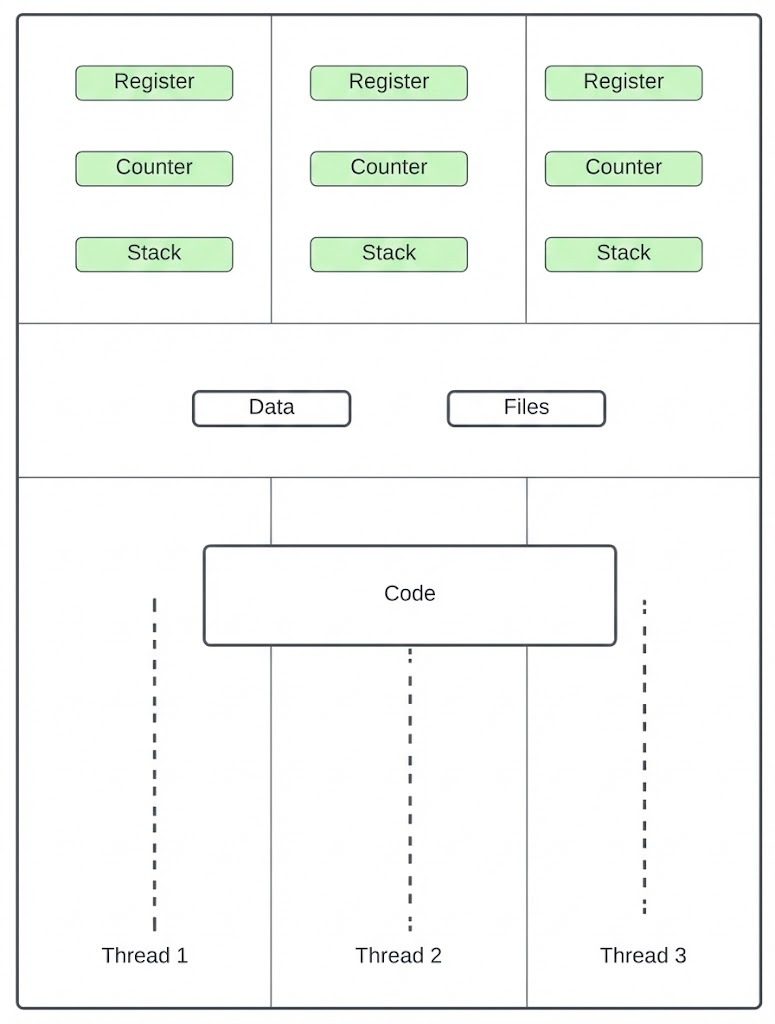
\includegraphics[scale = 0.4]{media/akshayintro3.png}
\caption{text}
\label{fig-akshayintro3}
\end{figure}




To achieve concurrent data acquisition and network transmission, the project utilizes the POSIX Threads (pthread) library. This library provides the primitives required to manage parallel execution paths within the Linux userspace. The specific functions utilized in this project are detailed below:

\subsection{Thread Management}
\begin{itemize}
    \item \texttt{pthread\_create( )}: Create a new thread
   	\begin{minted}[bgcolor = lightgray, tabsize = 4, breaklines]{c}
   	int pthread_create(pthread_t *thread, const pthread_attr_t *attr, void *(*start_routine)(void *), void *arg);
   	\end{minted}
    This function is the entry point for parallel execution. In this project,
    it is used in \texttt{main()} to spawn two critical worker threads: the
    Sensor Thread and the Server Thread. It takes the thread ID pointer,
    thread attributes (passed as \texttt{NULL} for default settings), and the
    function to execute (e.g., \texttt{sensor\_thread\_function}). A return
    value of zero indicates successful creation.

    \item \texttt{pthread\_join( )}: Wait for thread termination
    \begin{minted}[bgcolor = lightgray, tabsize = 4, breaklines]{c}
    int pthread_join(pthread_t thread, void **retval);
    \end{minted}
    This function is used by the main thread to wait for the worker threads to
    finish their execution. It acts as a blocking mechanism; the main program
    will not exit until the specified thread terminates. In this system, it
    ensures the application remains active and does not shut down prematurely
    while the sensors are still monitoring.
\end{itemize}

\subsection{Synchronization (Mutexes)}
Since multiple threads attempt to access shared resources, specifically the Ring Buffer for data storage and the Configuration Structure for settings synchronization is mandatory to prevent data corruption (Race Conditions). We utilize Mutexes (Mutual Exclusion objects) to enforce safe access.

\begin{itemize}
    \item \texttt{pthread\_mutex\_init( )}: Initialize the mutex
    \begin{minted}[bgcolor = lightgray, tabsize = 4, breaklines]{c}
int pthread_mutex_init(pthread_mutex_t *mutex, const pthread_mutexattr_t *attr);
    \end{minted}
    Called at the start of the program, this prepares the mutex object for
    use. It sets the mutex to an unlocked state, making it ready to manage
    resource contention.

    \item \texttt{pthread\_mutex\_lock( )}: Acquire the lock
    \begin{minted}[bgcolor = lightgray, tabsize = 4, breaklines]{c}
int pthread_mutex_lock(pthread_mutex_t *mutex);
    \end{minted}
    Before a thread can read or write to the shared Ring Buffer, it calls this
    function. If the buffer is currently free, the thread locks it and
    proceeds. However, if the other thread is already holding the lock, the
    calling thread is put to sleep (blocked) until the mutex becomes
    available. This guarantees atomic access to the data.

    \item \texttt{pthread\_mutex\_unlock( )}: Release the lock
    \begin{minted}[bgcolor = lightgray, tabsize = 4, breaklines]{c}
int pthread_mutex_unlock(pthread_mutex_t *mutex);
    \end{minted}
    Immediately after the data transfer is complete, the thread calls this
    function to release the mutex. This allows the waiting thread to wake up
    and access the shared resource.

    \item \texttt{pthread\_mutex\_destroy( )}: Clean up resources
    \begin{minted}[bgcolor = lightgray, tabsize = 4, breaklines]{c}
int pthread_mutex_destroy(pthread_mutex_t *mutex);
    \end{minted}
    Used during the system shutdown phase, this function destroys the mutex
    object, freeing any system resources associated with the lock mechanism.
\end{itemize}


\subsection{Sensor Thread}
This thread is exclusively responsible for precision timing and hardware data
acquisition. By offloading this workload, the main application is free to
handle TCP network communication and high-level client command logic, while
the sensor thread manages the low-level protocols required to extract accurate
temperature, ADC, and digital I/O readings.

The thread attempts to open the specific Linux device driver
(\texttt{/dev/meascdd}); if the physical hardware is not present, it
automatically falls back to a `Simulation Mode' that generates realistic sine
waves and dummy data. Inside its continuous execution loop, it calculates the
exact microsecond when the next sample is due for each individual sensor
(e.g., \texttt{next\_temp\_time}, \texttt{next\_adc0\_time}) using an Earliest
Deadline First approach rather than relying on fixed sleep intervals. When a
sensor's precise deadline is reached, the thread calls the specific reading
function (such as \texttt{TempRead} or \texttt{GetADC}) which interacts with
the hardware via a safe hardware-polling loop and then pushes the acquired data
and a microsecond timestamp into the thread-safe Ring Buffer to be processed
by the server thread.

This report details the architectural design, lifecycle management, data
acquisition strategies, and the synchronization mechanisms that constitute the
sensor thread.


\begin{figure}[H]
\centering 
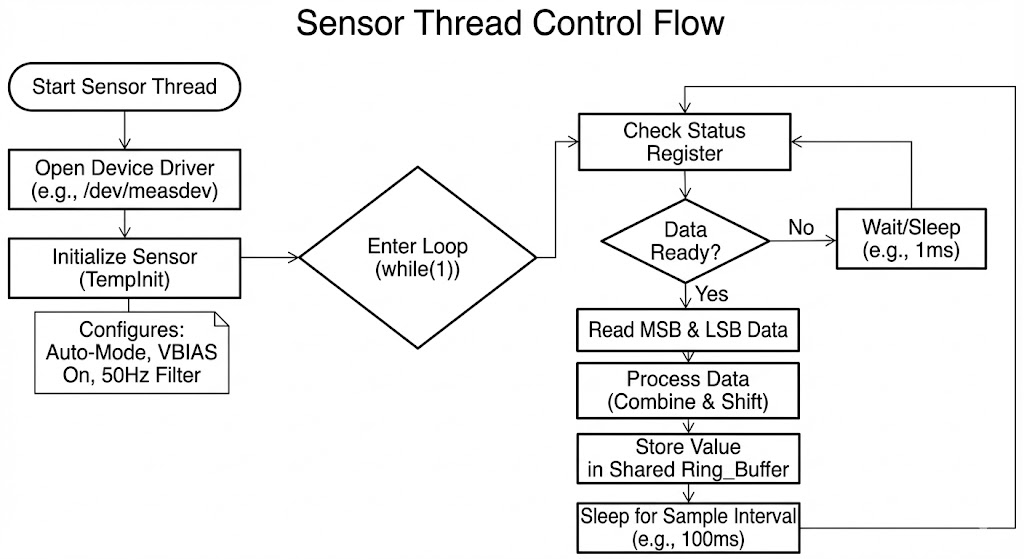
\includegraphics[width = 0.9\textwidth]{media/akshayintro7.png}
\caption{Flowchart Sensor thread control flow}
\label{fig-alshay7}
\end{figure}

The software architecture adopted for this project is a layered model designed
to abstract the complexities of hardware interaction from the application
logic. At the lowest level lies the physical hardware: the MAX31865 sensor
chip connected via SPI to the FPGA fabric of the Zynq SoC. Above this sits
the Linux Kernel Module (LKM), a device driver that exposes the hardware to
the operating system as a character device file, typically located at
\texttt{/dev/measdev}.

The Sensor Thread operates in the userspace layer, acting as the Hardware
Abstraction Layer (HAL). It communicates with the kernel driver using standard
POSIX file operations—specifically \texttt{open()}, \texttt{write()}, and
\texttt{read()}. This design choice is significant because it allows the
application to remain portable and relatively simple; the complex timing and
electrical signg required by the SPI bus are handled by the kernel driver
and the FPGA logic. The sensor thread's role is to construct the correct
command packets defined as \texttt{TF\_Obj\_Snd} for sending and
\texttt{TF\_Obj\_Rcv} for receiving that tell the driver which register to
access and what value to write. This transactional protocol ensures that the
application has fine-grained control over the sensor configuration without
needing direct access to physical memory addresses.

The lifecycle of the sensor thread is distinct from the main application,
following a rigorous sequence of initialization, execution, and termination.
Upon creation, the thread's first responsibility is to establish a
communication channel with the hardware. It does this by obtaining a file
descriptor to the device driver. This descriptor serves as a handle for all
subsequent interactions; if the driver cannot be opened, the thread must
handle this failure gracefully, typically by logging an error and exiting, as
the system cannot function without access to the sensor.

Once the connection is established, the thread enters the initialization
phase. The MAX31865 sensor defaults to a low-power ``sleep'' state upon
power-up and must be explicitly configured before it can perform any
conversions. The sensor thread executes a function, which sends a specific
sequence of commands to the sensor's Configuration Register (Address
\texttt{0x00}). The first command sets the VBIAS bit (Bit 7), which turns on
the DC bias voltage required to measure the resistance of the PT100 probe.
Without this voltage, the sensor would read effectively zero resistance. The
second critical command configures the internal digital filter. In industrial
environments, electrical noise from 50Hz mains power lines can couple into the
sensor wires, corrupting the sensitive analog measurements. The thread writes a
command to enable the 50Hz rejection filter, instructing the MAX31865 to
average its samples in a way that mathematically cancels out this specific
frequency interference. Finally, the thread sets the ``Auto Conversion'' bit,
switching the sensor from ``One-Shot'' mode to ``Continuous'' mode, where it
autonomously performs conversions in the background.


\begin{figure}[H]
\centering 
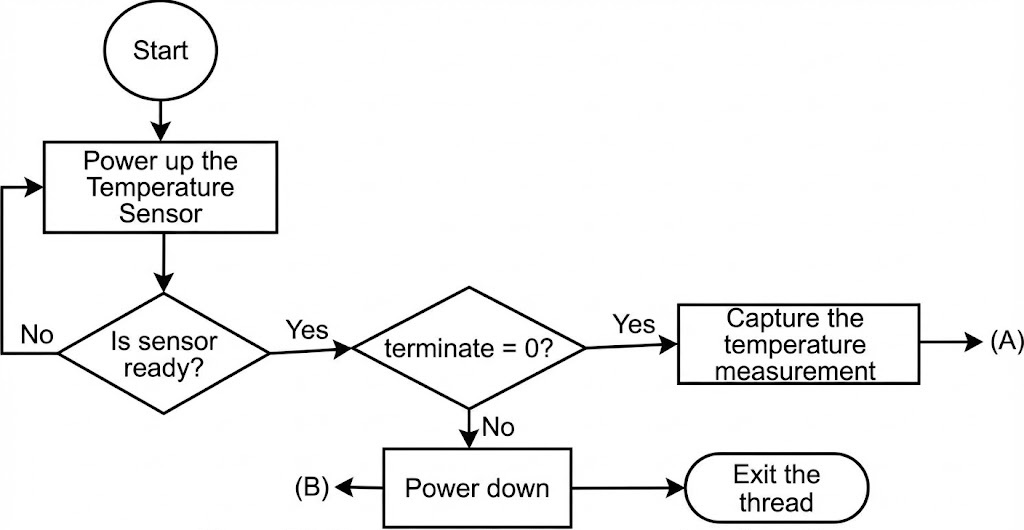
\includegraphics[width = 0.9\textwidth]{media/akshayintro2.png}
\caption{Flow chart of Temperature sensor thread}
\label{fig-akshayintro6}
\end{figure}

The provided flowchart illustrates the execution sequence for the temperature
sensor thread within the data acquisition system. The process begins at the
``Start'' state, immediately proceeding to a block instructing the system to
``Power up the Temperature Sensor''. Because the physical hardware requires a
brief period to initialize, the system enters a validation loop, querying the
condition ``Is sensor ready?''. If the sensor is not yet responsive, the loop
cycles back continuously until the hardware confirms its readiness.

Once the temperature sensor is fully operational, the thread evaluates a
critical control flag by asking if ``terminate = 0?''. This condition
determines whether the thread should continue its normal operation or begin a
shutdown sequence. If the flag indicates that no termination has been requested
(evaluating to ``Yes''), the thread proceeds to ``Capture the temperature
measurement''. After the data is successfully captured, the flow transitions
to a subsequent processing stage, which is indicated by the external connector
(A).

Alternatively, if a termination signal has been detected, the system halts any
further data measurements. It safely transitions to a shutdown routine to
``Power down'' the hardware components. After safely powering down the sensor,
the execution reaches its final conclusion at ``Exit the thread''.
Additionally, this secure power-down and exit sequence can also be triggered
via an external path labeled with connector (B).

\clearpage 
\subsection{ADC Sensor Thread}
\begin{figure}[H]
\centering 
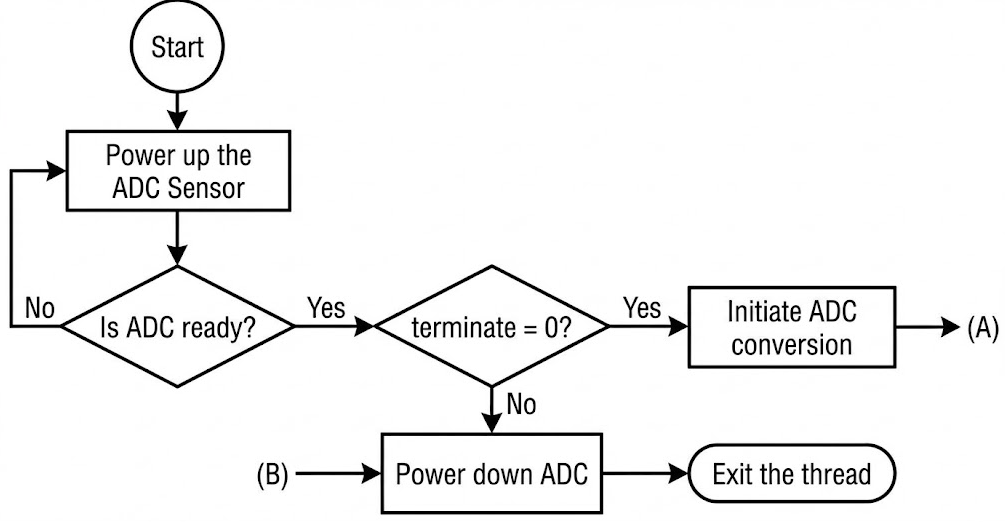
\includegraphics[width = 0.8\textwidth]{media/akshayintro6.png}
\caption{Flow chart of ADC sensor thread}
\label{fig-akshay6}
\end{figure}

The provided flowchart outlines the execution, hardware polling, and
termination logic for the Analog-to-Digital Converter (ADC) sampling sequence
within the embedded system's unified sensor thread.

The sequence begins by evaluating a core control condition, checking if the
thread's termination flag is equal to 0. This acts as the main execution
safeguard at the start of the thread's continuous loop. If the condition is
true, the system proceeds to issue a `Request Conversion' command to the ADC
hardware. Because hardware peripherals require time to sample analog voltage,
the system enters a polling loop that repeatedly asks, `Is the ADC ready?'.
If the hardware is not yet responsive, the loop continuously cycles back
safely yielding CPU time until a positive status confirmation is received from
the sensor driver.

Once the ADC confirms it has completed the conversion, the system reads the
raw data registers before moving to a subsequent processing and buffering
phase denoted by Connector (A).

Conversely, if the system receives a termination request, it immediately
aborts any further data sampling. It transitions directly to a safety sequence
to cleanly power down associated hardware and close the device file descriptors
before ultimately concluding with `Exit the thread'. Furthermore, this cleanup
block can also be accessed via an external path labeled with Connector (B),
ensuring that the hardware is always safely deactivated prior to thread
closure.

\subsection{Push Button Data Acquisition Strategy}
This system integrates the Push Button interface directly into the centralized Sensor Thread. This design choice eliminates the overhead of context switching between multiple threads and ensures deterministic sampling synchronization with the other sensors.

This flowchart illustrates the specific execution steps for acquiring data
from the digital Push Button sensors. It details the sequence of operations
that occur once the system determines it is time to sample the buttons.

\begin{itemize}
    \item \textbf{Capture Measurement Time:} The process begins by recording
    the current system timestamp. This ensures the data is temporally accurate
    for later analysis.

    \item \textbf{Read Push Button Values:} The system accesses the hardware
    register to retrieve the current state of the buttons. This involves a
    low-level register read followed by bitwise operations (shifting and
    masking) to isolate the specific bits representing the button states.

    \item \textbf{Calculate Relative Time:} The system calculates the time
    difference between the current measurement and the initial system start
    time. This relative timestamp is used to reduce the data size required for
    storage.

    \item \textbf{Data Storage (FIFO):} The combined data packet containing
    the button state and the timestamp is copied into the Ring Buffer. This
    makes the data available for the Server Thread to transmit.

    \item \textbf{Exit/Loop:} The flow then proceeds to exit the specific task
    or loop back, waiting for the next scheduled sampling interval or a
    termination signal.
\end{itemize}

\begin{figure}[H]
\centering 
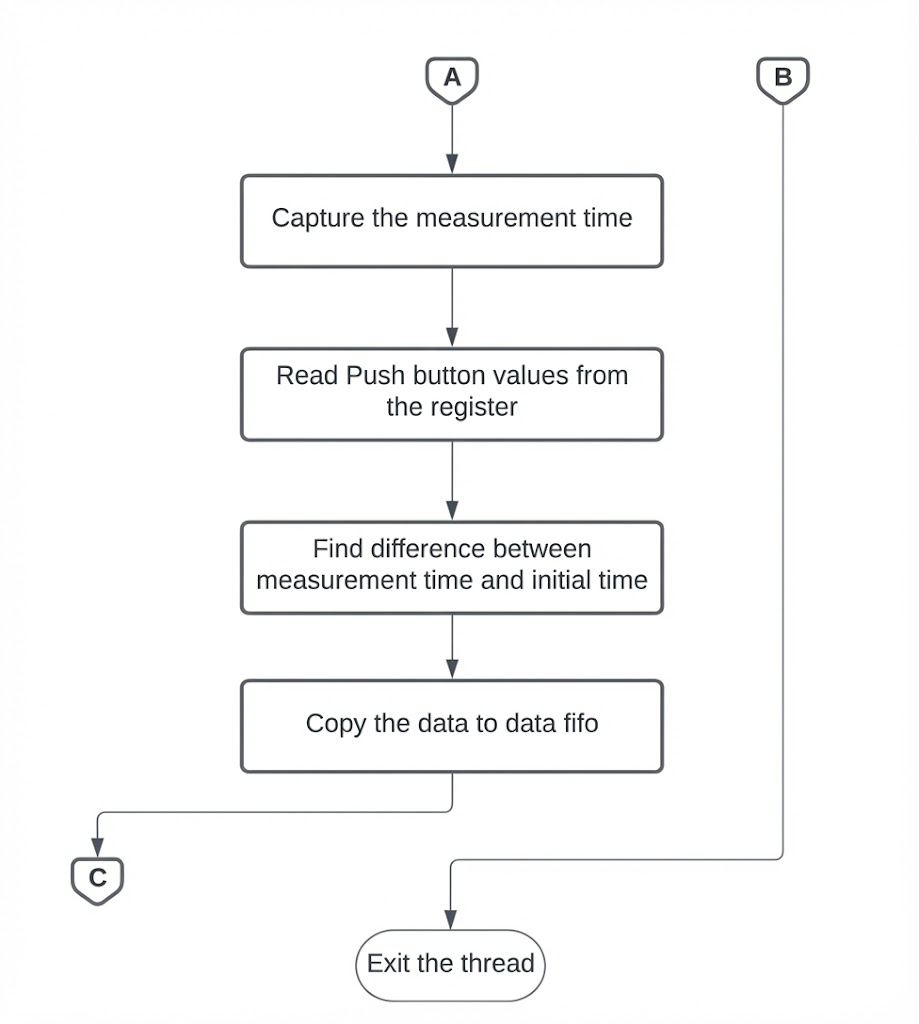
\includegraphics[width = 0.7\textwidth]{media/akshayintro4.png}
\caption{Flow chart of push button and switches thread}
\label{fig-akshay4}
\end{figure}

\subsection{The Data Acquisition Loop}
The core operational logic of the sensor thread is contained within an infinite while(1) loop. Rather than a simple continuous polling mechanism, this loop acts as a highly precise scheduler, utilizing an "Earliest Deadline First" approach to independently manage multiple sensors. When the exact microsecond deadline arrives for a temperature reading, the thread enters the hardware-specific data retrieval phase.

It initiates a 1-shot conversion and queries the sensor via the custom device driver. To prevent reading stale data while the MAX31865 completes its conversion, the thread inspects the status response from the hardware. It looks for a specific ready state, If the hardware is not yet ready, the thread performs a safe "busy wait," utilizing a function to yield the processor to the OS for 10 microseconds, preventing the CPU from spinning at 100\% utilization.

Once the ready state is confirmed, the thread proceeds to read the two data registers: the Most Significant Byte (MSB) at Address 1 and the Least Significant Byte (LSB) at Address 2. These two 8-bit values must be combined to form the complete 16-bit raw temperature reading. The thread performs this combination using bitwise operations, shifting the MSB left by 8 positions and performing a bitwise OR with the LSB.


\subsection{Data Processing and Fault Management}
The raw 16-bit integer retrieved from the MAX31865 is not yet a valid temperature value. The chip encodes fault information directly into the least significant bit (Bit 0) of the data word, acting as a flag to indicate hardware faults such as an open circuit or a short circuit in the RTD probe.

However, in this specific gateway architecture, the embedded C application prioritizes maximum throughput and deterministic latency. Therefore, the sensor thread does not locally perform the right-shift operations to isolate the fault bit, nor does it calculate the complex floating-point. Instead, the gateway acts as a transparent, high-speed conduit. It immediately pushes the pristine, raw 16-bit integer directly into the Ring Buffer. This architectural decision deliberately delegates the heavy mathematical conversions and fault-flag evaluations to the higher-level client dashboard receiving the TCP stream, keeping the embedded gateway incredibly lightweight, fast, and stable.

\subsection{Thread Synchronization and Shared Memory}
One of the most critical aspects of the sensor thread's design is how it safely shares data with the rest of the system. Since the sensor thread runs asynchronously to the TCP server thread, direct variable access would inevitably lead to "race conditions," where the server might read a corrupted value such as a mix of an old MSB and a new LSB.

To solve this, the system employs a robust Ring Buffer mechanism. The sensor thread acts as the "Producer," pushing valid, timestamped sensor readings into the buffer. The dedicated server thread acts as the "Consumer," reading these values to batch and transmit over the network.

This shared memory access is strictly protected by Mutex locks. The sensor thread locks the mutex before writing to the buffer and unlocks it immediately after, guaranteeing that the write operation is atomic and cannot be interrupted. Furthermore, the system implements advanced event-driven synchronization using a Condition Variable. Instead of the server thread wasting CPU cycles continuously polling the buffer to see if new data has arrived, it enters a deep sleep. The exact microsecond the sensor thread finishes a safe write, it fires a signal that instantly wakes the server thread to process the data.\\

\textbf{Client-Side Data Processing and GUI Visualization}

To maintain maximum throughput and minimize CPU overhead on the embedded
ZedBoard gateway, heavy mathematical computations and data unpacking are
deliberately offloaded to the remote client application. The client dashboard,
operating on a standard PC, connects to the gateway via a TCP socket and
continuously ingests the incoming byte stream.\\

\textbf{Data Parsing and Fault Masking}

Upon receiving the raw 16-bit integer generated by the MAX31865 sensor, the
client software first evaluates the least significant bit (Bit 0), which
serves as a hardware fault flag. If this bit is asserted (1), the client
triggers a graphical user interface (GUI) alert indicating a potential open
circuit or short circuit in the RTD probe. If the bit is clear (0), the
software performs a logical right-shift operation to discard the status bit,
successfully isolating the true 15-bit ADC count.\\

\textbf{Mathematical Conversion and Rendering}

The isolated raw integer represents the physical ratio of the RTD resistance
to the reference resistor. The client application then applies the
Callendar-Van Dusen equation to convert this raw resistance ratio into a
precise, human-readable floating-point temperature value in degrees Celsius.

Once processed, the temperature, alongside the decoded ADC voltages and
digital switch states, is pushed to the graphical platform. The dashboard
dynamically updates real-time plots and status indicators, providing operators with an intuitive, lag-free overview of the distant sensor nodes. This architectural decision keeps the embedded gateway incredibly lightweight and fast, while leveraging the superior processing power of the client PC for complex mathematics and UI rendering.

\subsection{Results and System Validation}
To verify the stability, concurrency, and network capabilities of the Measurement Network Gateway, extensive testing was conducted directly on the physical Xilinx Zynq-7000 SoC (ZedBoard).

The system's initialization sequence and hardware abstraction layer were thoroughly validated. The sensor thread successfully opened the custom /dev/meascdd Linux device driver and established SPI communication with the physical MAX31865 and ADC peripherals. The thread correctly transmitted the configuration bytes to enable the VBIAS and the 50Hz hardware noise filter. Monitoring the system confirmed that the continuous polling loop accurately retrieved real, fluctuating analog readings at the exact microsecond intervals dictated by the Earliest Deadline First scheduling algorithm.

The TCP/IP server thread was validated by connecting the custom graphical platform (GUI) to the gateway over the local network. The server successfully maintained the connection and accurately processed the custom command protocol (e.g., start, stop, configure). Once the stream was initiated, the GUI successfully ingested the raw 16-bit integers, masked the hardware fault bits, and applied the Callendar-Van Dusen equation. The dashboard dynamically updated the real-time plots and status indicators with accurate temperature and voltage readings, proving that the gateway's deliberate architectural choice to offload heavy mathematics to the client was highly effective.

Finally, the system was stress-tested to ensure the POSIX synchronization primitives functioned under continuous load. The concurrent Producer-Consumer architecture proved completely stable; the server thread managed network flow control and client communication without ever interrupting or blocking the underlying sensor data acquisition thread. The Mutex-protected Ring Buffer and POSIX Condition Variables successfully facilitated data exchange with zero dropped packets and near-zero CPU waste during idle states. Even when network latency was introduced or the client was intentionally disconnected, the sensor thread continued acquiring data uninterrupted, successfully preventing data loss and system hangs.

\subsection{Conclusion}
The Sensor Thread implementation detailed in this report represents a robust
and scalable solution for embedded data acquisition on the Xilinx ZedBoard
platform. By encapsulating hardware complexity within a dedicated,
high-performance thread, the system achieves a modular architecture where the
low-level intricacies of SPI communication and register manipulation are
completely abstracted from the high-level TCP server logic.

The thread manages the comprehensive lifecycle of multiple sensors. For the
temperature hardware, this ranges from the critical initialization sequence
which powers up the VBIAS and enables hardware-level noise filtering to the
precision-timed, continuous loops that retrieve the raw data. While the
hardware-to-thread interaction relies on a highly optimized, yielded polling
design (involving minor trade-offs in strict real-time determinism), the
thread-to-thread communication is fully event-driven. The implementation of a
Mutex-protected Ring Buffer paired with POSIX Condition Variables ensures safe,
reliable, and zero-CPU-waste data exchange with the main server application.

Ultimately, this architecture provides a highly stable and lightweight
foundation for industrial IoT monitoring systems, maintaining clear pathways
for future hardware-level optimizations via kernel-space wait queues and
hardware interrupt handling.